\section{Experiments over 2 axes}
The previous study show the link between the precision and the complexity of the abstraction that we used.
In this part we will use the previous results in order to solve the following problem for different size of the environment.
\begin{figure}
	\center
	\includestandalone[width=0.5\textwidth]{2D_env_problem}
	\caption{Testing environment for the quadricopter.}
	\label{fig:environment}
\end{figure}

\comment{Show the simulation, the runs and so on.}

\subsection{$\Ninputs = 1$ input memory model}
See figure \ref{fig:double_reduce_2D}.

\begin{figure*}
	\center
	\includestandalone[width=\textwidth]{double_reduced_2D}
	\caption{$\Ninputs=1$ input memory model in 2D.}
	\label{fig:double_reduce_2D}
\end{figure*}


\subsection{Real case scenarios}
See figure \ref{fig:real_case}.
In the case of the wind turbine application, the quad will have to go from the base station to the wind turbine blade and explore a given set of regions while avoiding the blade.
The wind can be modelled as a perturbation on the velocity of the quadricopters.
We have been using the first integrator model in this case.

\begin{figure}[!ht]
  \centering
  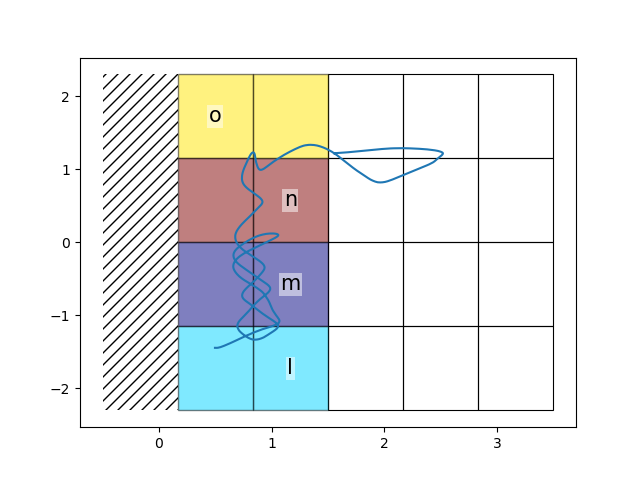
\includegraphics[width=0.9\linewidth]{real_case_scenarios}
  \caption{A trajectory in the state space $(x,v)$.}
  \label{fig:real_case}
\end{figure}

